\chapter{Rush Hour Intervention Human Subject Experiment}
\label{apx:rushintervention}
We discuss details about the Rush Hour human subject study and the findings. The following sections present the evidence on which we based the design choices for the Rush Hour planning task. The sections are cross-referenced throughout the main content.

\section{Rush Hour Human Subject Study: Pilot Experiment}
\label{ap:pilot}
Before the study was actually administered to our recruited subjects, a pilot study was conducted with nine graduate students to assess whether they would be able to solve the puzzles within a reasonable amount of time. The pilot study participants solved their assigned puzzles within 5-10 minutes. The pilot study participants were also interviewed informally to get their perception of the puzzle difficulty. The participants commented that the puzzles were ``\textit{challenging}'' and ``\textit{forced me to think}''. The same puzzles used in the pilot were used in the actual study.\\

\section{Experimental Design}
\label{ap:phase1design}
For the actual study, we recruited subjects from a university student population. 
The participants were not compensated for their time. 
After obtaining informed consent, the participants were directed to the Web URL, which hosted the Rush Hour Web Simulator. 
Each participant was assigned to solve one Rush Hour puzzle randomly selected from a set of ten. 
We did not place any time restriction for the puzzle solving task. 
Participants also had the option to use an online tutorial. 
All ten puzzles contained a forbidden vehicle. 
The participants were informed that one of the vehicles on the game board is forbidden and the puzzle must be solved without moving the forbidden vehicle. 
However, in this phase we did not give any visual cues (error messages, blocks, intervention) to the user in case they happen to move the forbidden vehicle during game play. 
Once the puzzle solving task was completed, the participants were asked to complete a short demographic survey on their general puzzle solving habits. 
Figure \ref{fig:phase1} illustrates the activity sequence of the experiment. 136 participants completed the study. The sample comprised of college undergraduate and graduate students in Computer Science, Psychology, Agriculture and Business majors. 117 of the 136 participants also completed the demographics survey.

\begin{figure}[tpb]
  \centering                                                    
  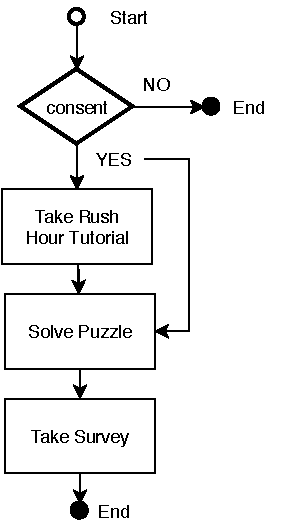
\includegraphics[keepaspectratio]{img/phase1.pdf}
  \caption{Activity sequence for learning when to intervene human subject experiment}
  \label{fig:phase1}
\end{figure}

\section{Demography Survey Findings}
\label{ap:demographics}
Majority of the participants (39) were below the age of 20, while 38 subjects were between the age 20-25. Maximum age was 41 years. 70 of the 117 participants were male. When asked if they liked puzzle solving tasks, 78\% of the participants either agreed or strongly agreed with the statement. Specifically to the Rush Hour game 79\% of the participants liked or strongly liked Rush Hour. The most common reason as to why the participants liked puzzle solving tasks was that puzzle solving stimulates critical thinking skills. 30\% of the participants usually did a puzzle solving task once a month, while 21\% of the participants solved a puzzle once a week. When asked about strategies the participants used to solve difficult puzzles, 79\% of the group said that they kept trying until the puzzle was eventually solved, while 12\% of the participants said that they would ask for help. 

Given a new puzzle that they have not seen before, if they get stuck while solving the puzzle, 26\% said that they would not like any outside help. 47\% of the participants said that they would like a suggestion/tip that would get them past the current situation. 15\% said that they would like a warning, which indicated that their current approach would lead to a dead-end. 8\% of the participants said that they would like a warning and an explanation to help them prevent getting stuck in the future.  The most common medium for solving puzzles was using their mobile devices (42\%). 31\% of the participants used the personal computers/laptops to solve puzzles. 19\% of the participants solved puzzles using physical means (e.g., puzzle books, newspapers and physical puzzles such as Rubik's  cubes).\\

\section{User Solutions Grouped by Length}
\label{ap:lengroups}
For each puzzle, we sorted the solutions by the number of moves (in the complete solution) in the ascending order and split them into three groups (fast, medium, slow). We ensured that the three groups for each puzzle contained approximately equal number of users. Table \ref{tab:solvergroups} summarizes the findings. There were 46 users in the fast group, 42 in the medium and 48 in the slow group. Mean refers to the mean number of moves in a solution produced by users who solved a specific puzzle. Forbidden moves refers to the number of times, the users who solved a specific puzzle moved the forbidden vehicle.

\begin{table}[ptb]
\caption{Plans produced by human users grouped by the mean number of moves and the number of forbidden moves}
\label{tab:solvergroups}
\begin{tabular}{|l|l|l|l|l|l|l|}
\hline
\multicolumn{1}{|c|}{\multirow{2}{*}{PID}} &
  \multicolumn{2}{c|}{Fast (46)} &
  \multicolumn{2}{c|}{Medium (42)} &
  \multicolumn{2}{c|}{Slow (48)} \\ \cline{2-7} 
\multicolumn{1}{|c|}{} &
  \multicolumn{1}{c|}{Mean} &
  \multicolumn{1}{c|}{\begin{tabular}[c]{@{}c@{}}Forbidden\\ Moves\end{tabular}} &
  \multicolumn{1}{c|}{Mean} &
  \multicolumn{1}{c|}{\begin{tabular}[c]{@{}c@{}}Forbidden\\ Moves\end{tabular}} &
  \multicolumn{1}{c|}{Mean} &
  \multicolumn{1}{c|}{\begin{tabular}[c]{@{}c@{}}Forbidden\\ Moves\end{tabular}} \\ \hline
P1  & 25.5 & 0  & 41.7  & 0  & 64.7  & 0  \\ 
P2  & 74.7 & 4  & 137.7 & 16 & 277   & 28 \\ 
P3  & 26.5 & 8  & 36.2  & 9  & 43.7  & 6  \\ 
P4  & 25.2 & 1  & 32    & 4  & 76    & 28 \\ 
P5  & 18.3 & 3  & 26    & 2  & 44.75 & 13 \\ 
P6  & 22   & 0  & 24.5  & 0  & 39.6  & 0  \\ 
P7  & 38.5 & 5  & 53.3  & 16 & 120   & 37 \\ 
P8  & 9    & 0  & 9     & 0  & 10    & 0  \\ 
P9  & 27.8 & 8  & 48.6  & 12 & 99    & 28 \\ 
P10 & 50.3 & 11 & 66    & 14 & 127.3 & 46 \\ \hline
\end{tabular}
\end{table}